\documentclass[11pt,oneside]{report}

\usepackage[T1]{fontenc}
\usepackage[utf8]{inputenc}
\usepackage{lmodern}
\usepackage[letterpaper,margin=0.82in,headheight=14pt]{geometry}
\usepackage{microtype}
\usepackage{xcolor}
\usepackage{graphicx}
\usepackage{booktabs}
\usepackage{longtable}
\usepackage{tabularx}
\usepackage{array}
\usepackage{amsmath}
\usepackage{amssymb}
\usepackage{mathtools}
\usepackage{enumitem}
\usepackage{listings}
\usepackage{tikz}
\usetikzlibrary{arrows.meta,positioning,calc,fit}
\usepackage{float}
\usepackage{placeins}
\usepackage{hyperref}
\usepackage{fancyhdr}

\definecolor{navy}{HTML}{17365D}
\definecolor{blue}{HTML}{2F75B5}
\definecolor{lightblue}{HTML}{EAF2F8}
\definecolor{green}{HTML}{548235}
\definecolor{lightgreen}{HTML}{EAF4E3}
\definecolor{orange}{HTML}{C55A11}
\definecolor{lightorange}{HTML}{FFF2CC}
\definecolor{red}{HTML}{A61C00}
\definecolor{lightred}{HTML}{FCE8E6}
\definecolor{graytext}{HTML}{4A4A4A}
\definecolor{codebg}{HTML}{F5F7F9}
\definecolor{rulegray}{HTML}{D9E1E8}

\hypersetup{
  colorlinks=true,
  linkcolor=navy,
  urlcolor=blue,
  citecolor=green,
  pdftitle={Forward-emulator handbook: model c 2in 1out new channels p cont BT loss v1},
  pdfauthor={Code-authoritative repository handbook},
  pdfsubject={Training, validation, inference, FNO architecture, tests, and Slurm operation}
}

\pagestyle{fancy}
\fancyhf{}
\fancyhead[L]{Forward-emulator handbook}
\fancyhead[R]{\nouppercase{\leftmark}}
\fancyfoot[C]{\thepage}
\renewcommand{\headrulewidth}{0.4pt}

\setcounter{secnumdepth}{3}
\setcounter{tocdepth}{2}
\setlist[itemize,enumerate]{nosep,leftmargin=*}
\setlist[description]{nosep}
\setlength{\parindent}{0pt}
\setlength{\parskip}{0.55em}
\renewcommand{\arraystretch}{1.18}

\lstdefinestyle{code}{
  backgroundcolor=\color{codebg},
  basicstyle=\ttfamily\small,
  breaklines=true,
  breakatwhitespace=false,
  columns=fullflexible,
  keepspaces=true,
  frame=single,
  rulecolor=\color{rulegray},
  showstringspaces=false,
  tabsize=2,
  xleftmargin=0.2em,
  xrightmargin=0.2em
}
\lstset{style=code}

\newcommand{\modelid}{\texttt{\detokenize{model_c_2in_1out_new_channels_p_cont_BT_loss_v1}}}
\newcommand{\repo}[1]{\nolinkurl{#1}}
\newcommand{\code}[1]{\texttt{\detokenize{#1}}}
\newcommand{\R}{\mathbb{R}}
\newcommand{\Ltwo}{L^2}
\newcommand{\eps}{\varepsilon}
\newcommand{\important}[1]{%
  \par\medskip\noindent
  \fcolorbox{red}{lightred}{%
    \parbox{\dimexpr\textwidth-2\fboxsep-2\fboxrule\relax}{\textbf{Important.} #1}}%
  \par\medskip}
\newcommand{\operational}[1]{%
  \par\medskip\noindent
  \fcolorbox{orange}{lightorange}{%
    \parbox{\dimexpr\textwidth-2\fboxsep-2\fboxrule\relax}{\textbf{Operational note.} #1}}%
  \par\medskip}
\newcommand{\verified}[1]{%
  \par\medskip\noindent
  \fcolorbox{green}{lightgreen}{%
    \parbox{\dimexpr\textwidth-2\fboxsep-2\fboxrule\relax}{\textbf{Verified.} #1}}%
  \par\medskip}
\newcommand{\safegraphic}[2][]{%
  \IfFileExists{#2}{%
    \includegraphics[#1]{#2}%
  }{%
    \fbox{\parbox{0.88\linewidth}{\centering
      Figure file not found at compile time:\par
      \nolinkurl{#2}}}%
  }%
}

\begin{document}
\hypersetup{pageanchor=false}

\begin{titlepage}
  \centering
  \vspace*{1.0cm}
  {\Huge\bfseries Forward Ocean Emulator\par}
  \vspace{0.55cm}
  {\Large\bfseries Hands-on training, validation, inference, and architecture handbook\par}
  \vspace{0.9cm}
  {\large \modelid\par}
  \vspace{1.1cm}
  \begin{tikzpicture}
    \node[
      draw=navy,
      fill=lightblue,
      rounded corners=4pt,
      line width=0.8pt,
      text width=0.84\textwidth,
      inner sep=12pt,
      align=left
    ] {
      \textbf{Scope.} This document describes only the retained forward emulator
      and the code paths that produced the artifacts grouped under
      \repo{outputs/af_fno/C/model_c_2in_1out_new_channels_p_cont_BT_loss/}.
      The adjoint study and \repo{archive/} are deliberately out of scope.
      Existing documents in \repo{docs/} were not used as technical sources.
    };
  \end{tikzpicture}
  \vfill
  {\large Code-authoritative snapshot: 14 August 2026\par}
  \vspace{0.25cm}
  {\small Repository: \repo{/home/mjalabert314/bire_james25_repro}\par}
  \vspace{0.55cm}
  {\small
    Intended reader: an intern who needs to reproduce, inspect, test, or safely
    modify the final forward model.
  \par}
\end{titlepage}

\hypersetup{pageanchor=true}
\pagenumbering{roman}
\tableofcontents
\clearpage

\chapter*{How to use this handbook}
\addcontentsline{toc}{chapter}{How to use this handbook}

This is an implementation manual, not a conceptual proposal. Statements about
the model are derived from the active Python modules in \repo{src/oceanfno/},
the three active forward contracts in \repo{config/}, the forward tests in
\repo{tests/}, the matching Slurm launchers, and the retained run artifacts.
Where a generated README conflicts with active code, this handbook follows the
code and contract.

The quickest reading paths are:

\begin{itemize}
  \item To run the existing workflow, read Chapters~\ref{ch:quickstart},
        \ref{ch:contracts}, and \ref{ch:slurm}.
  \item To understand the network, read Chapters~\ref{ch:data},
        \ref{ch:architecture}, and \ref{ch:rollout}.
  \item To modify training, read Chapters~\ref{ch:loss},
        \ref{ch:training}, \ref{ch:tests}, and \ref{ch:maintenance}.
  \item To interpret the retained figures, read Chapters~\ref{ch:validation}
        and \ref{ch:inference}.
\end{itemize}

\important{The exact checked-out launch contracts are historical, sealed
contracts, not safe scratch pads. Their project artifacts were moved one
directory deeper while the contracts retained the old direct paths, and their
scratch outputs still exist. The engines refuse overwrite. Do not submit the
three active \code{.sbatch} files blindly; first follow
Section~\ref{sec:current-checkout} and choose whether to inspect the retained run
or create a fresh versioned run.}

\clearpage
\pagenumbering{arabic}

\chapter{System at a glance}
\label{ch:overview}

\section{Scientific mapping}

The emulator advances a normalized, three-dimensional ocean state by ten days:
\begin{equation}
  F_\theta:
  \left(x_{t-10},x_t,s\right)
  \longmapsto \widehat{x}_{t+10}.
\end{equation}
The two input states supply a 20-day temporal context. The static block \(s\)
contains surface forcing, the land--ocean mask, and grid/forcing descriptors.
The output is the \emph{absolute normalized future state}; it is not an
increment and the implementation does not add \(x_t\) to the output.

At each grid point the state has 46 channels:
15 zonal velocities, 15 meridional velocities, 15 potential temperatures, and
one free-surface height. The grid is \(62\times62\). One call therefore maps
\[
  \R^{N\times97\times62\times62}
  \longrightarrow
  \R^{N\times46\times62\times62}.
\]

\section{End-to-end workflow}

\begin{figure}[H]
\centering
\resizebox{\textwidth}{!}{%
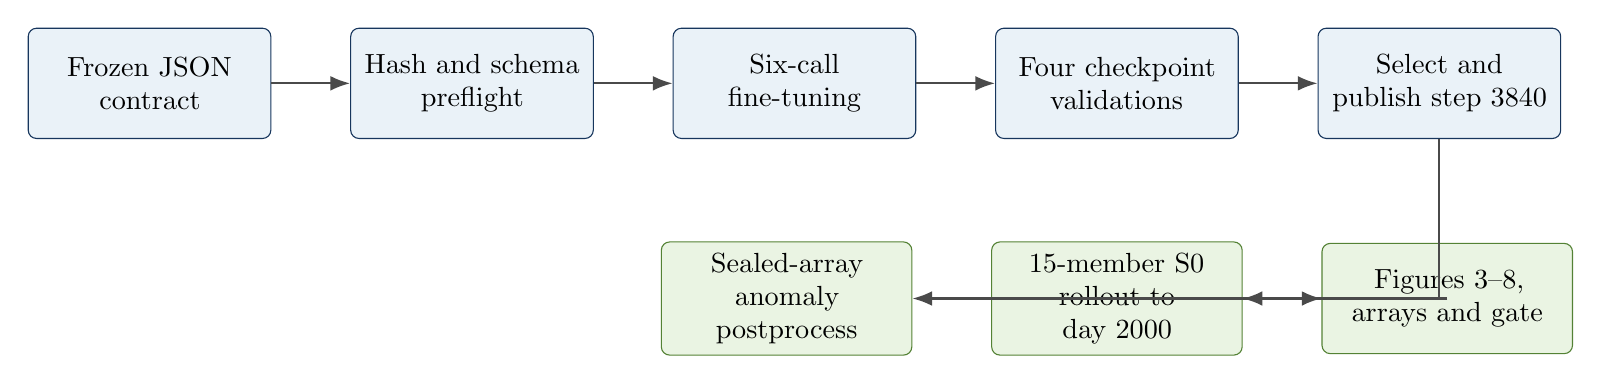
\begin{tikzpicture}[
  node distance=10mm,
  stage/.style={
    draw=navy, fill=lightblue, rounded corners=3pt,
    minimum height=14mm, text width=28mm, align=center, inner sep=4pt
  },
  post/.style={
    draw=green, fill=lightgreen, rounded corners=3pt,
    minimum height=14mm, text width=29mm, align=center, inner sep=4pt
  },
  arrow/.style={-{Latex[length=2.5mm]}, line width=0.8pt, color=graytext}
]
  \node[stage] (contract) {Frozen JSON\\contract};
  \node[stage, right=of contract] (preflight) {Hash and schema\\preflight};
  \node[stage, right=of preflight] (train) {Six-call\\fine-tuning};
  \node[stage, right=of train] (valid) {Four checkpoint\\validations};
  \node[stage, right=of valid] (select) {Select and\\publish step 3840};
  \node[post, below=13mm of valid] (figures) {15-member S0\\rollout to day 2000};
  \node[post, right=of figures] (products) {Figures 3--8,\\arrays and gate};
  \node[post, left=of figures] (anomaly) {Sealed-array\\anomaly postprocess};
  \draw[arrow] (contract) -- (preflight);
  \draw[arrow] (preflight) -- (train);
  \draw[arrow] (train) -- (valid);
  \draw[arrow] (valid) -- (select);
  \draw[arrow] (select) |- (figures);
  \draw[arrow] (figures) -- (products);
  \draw[arrow] (products) |- (anomaly);
\end{tikzpicture}}
\caption{Maintained forward workflow. Inference is implemented by the figure
stage; there is no separate general-purpose inference CLI. The anomaly stage
reads sealed rollout arrays and does not load the model.}
\label{fig:pipeline}
\end{figure}

\section{What is special about this version}

\modelid is a loss-only successor of
\repo{model_c_2in_1out_new_channels_pressure_gradient_continuity_v1}.
It strict-loads that parent's selected step-3840 model state, reuses its
normalization, discards the parent's Adam state, and performs 3,840 new updates.
The architecture is unchanged. The only new scientific objective is a
barotropic-transport increment loss with weight \(0.05\).

This distinction prevents three common misreadings:

\begin{enumerate}
  \item Step 3840 in the final report means 3,840 fine-tuning updates, not a
        cumulative label of 7,680;
  \item the local convolution is initialized to zero only in a fresh
        constructor, but this run immediately loads nonzero trained parent
        weights;
  \item the selected and comparator models in Figure~6 have the same five
        physical static channels. They differ by the added loss and resulting
        fine-tuning, not by architecture.
\end{enumerate}

\chapter{Quick start and current-checkout status}
\label{ch:quickstart}

\section{Repository and environment}

Run commands from the repository root:
\begin{lstlisting}
cd /home/mjalabert314/bire_james25_repro
bash scripts/bootstrap_env.sh
\end{lstlisting}

The bootstrap script creates \repo{.venv/}, installs PyTorch 2.6.0 for CUDA
12.4, and installs the editable project with the \code{fno} and \code{dev}
extras. Supported Python is 3.11--3.12. The model depends on
\code{neuraloperator==2.0.0}; the active runtime checks this exact version
because block ordering and defaults are part of the architecture contract.

\operational{The bootstrap script loads GNU 14.2, while production Slurm jobs
load GNU 12.2. The retained environment worked, but this compiler-module
difference is a portability/ABI risk when rebuilding binary packages. Record
\code{python --version}, \code{torch.__version__}, CUDA availability, and the
resolved dependency file for a new environment.}

\section{Read-only preflight}

Training preflight is non-mutating and currently succeeds:
\begin{lstlisting}
./.venv/bin/python -m oceanfno.train preflight \
  --contract config/model_c_2in_1out_new_channels_p_cont_BT_loss_v1.json
\end{lstlisting}

The equivalent figure and anomaly preflights are:
\begin{lstlisting}
./.venv/bin/python -m oceanfno.figures preflight \
  --contract config/model_c_2in_1out_new_channels_p_cont_BT_loss_s0_figures_v1.json

./.venv/bin/python -m oceanfno.anomaly preflight \
  --contract config/model_c_2in_1out_new_channels_p_cont_BT_loss_s0_anomaly_v1.json
\end{lstlisting}

In the current checkout, those last two commands fail because their pinned
project paths no longer point to the relocated retained packages. That failure
is expected and is not evidence that the checkpoint or numerical results are
bad.

\section{Current-checkout path mismatch}
\label{sec:current-checkout}

The JSON contracts name direct roots under
\repo{outputs/af_fno/C/}, for example:
\begin{lstlisting}
outputs/af_fno/C/model_c_2in_1out_new_channels_p_cont_BT_loss_v1
outputs/af_fno/C/model_c_2in_1out_new_channels_p_cont_BT_loss_s0_figures_v1
outputs/af_fno/C/model_c_2in_1out_new_channels_p_cont_BT_loss_s0_anomaly_v1
\end{lstlisting}

The retained packages now live one level deeper:
\begin{lstlisting}
outputs/af_fno/C/model_c_2in_1out_new_channels_p_cont_BT_loss/
  model_c_2in_1out_new_channels_p_cont_BT_loss_v1/
  model_c_2in_1out_new_channels_p_cont_BT_loss_s0_figures_v1/
  model_c_2in_1out_new_channels_p_cont_BT_loss_s0_anomaly_v1/
\end{lstlisting}

At the same time, canonical scratch directories under
\repo{/bigscratch/mjalabert314/bire_james25_repro/af_fno/models/C/} remain
populated. Training, figure generation, and anomaly generation all reject an
existing final directory or staging \code{.tmp} directory.

Choose one of these two modes:

\begin{description}
  \item[Inspect the retained run.] Read the grouped output paths above and the
  canonical scratch artifacts. If exact contract preflight is required,
  reconcile the expected direct paths with non-destructive links after checking
  every target. Do not call \code{run}; linked existing outputs will still
  trigger overwrite protection.

  \item[Create a new run.] Copy each JSON contract to a new versioned filename,
  change its version and both output roots to unused paths, point downstream
  artifacts at the new upstream report/checkpoint, and use the wrapper's
  \code{finalize} command where pending digests are supported. Preserve the
  old scratch and project roots as provenance.
\end{description}

\important{Do not fix this by changing a digest to match an arbitrary file.
First decide which artifact is authoritative, verify its identity, then update
path and digest together in a new contract. The contract is a scientific
record, not merely a runtime settings file.}

\section{Canonical Slurm sequence}

After preparing valid, unused output roots, submit:
\begin{lstlisting}
TRAIN_JOB=$(sbatch --parsable \
  slurm/models/c/train_2in_1out_new_channels_p_cont_BT_loss.sbatch)

FIGURE_JOB=$(sbatch --parsable --dependency=afterok:$TRAIN_JOB \
  slurm/models/c/figures_2in_1out_new_channels_p_cont_BT_loss.sbatch)

sbatch --dependency=afterok:$FIGURE_JOB \
  slurm/models/c/anomaly_2in_1out_new_channels_p_cont_BT_loss.sbatch
\end{lstlisting}

The launchers accept \code{AF_PROJECT_ROOT}, \code{AF_CONTRACT}, and
\code{AF_PYTHON}. Prefer these overrides when testing a copied contract so
that the retained launcher remains unchanged.

\chapter{Data contract and preprocessing}
\label{ch:data}

\section{Trajectory store}

The active training contract pins:
\begin{lstlisting}
/bigscratch/mjalabert314/bire_james25_repro/af_fno/datasets/trajectories_v3.zarr
\end{lstlisting}

Its central state array is float32 with shape
\((3,9000,46,62,62)\) and chunks \((1,8,46,62,62)\). The first axis holds
three forcing regimes, S0--S2. Chunk-aware batching keeps nearby records
together to reduce Zarr reads, then deterministically shuffles the batch order.

\begin{table}[H]
\centering
\caption{State channel order. This order is a hard interface shared by the
dataset, network, diagnostic functions, and physics losses.}
\begin{tabularx}{\textwidth}{@{}lrrX@{}}
\toprule
Group & Python slice/index & Count & Physical quantity \\
\midrule
\(U\) & \code{0:15} & 15 & Zonal velocity, levels \code{U_01}--\code{U_15} \\
\(V\) & \code{15:30} & 15 & Meridional velocity, levels \code{V_01}--\code{V_15} \\
\(\Theta\) & \code{30:45} & 15 & Potential temperature, levels \code{Theta_01}--\code{Theta_15} \\
\(\eta\) & \code{45} & 1 & Free-surface height, \code{Eta} \\
\bottomrule
\end{tabularx}
\end{table}

\section{Effective temporal split}

The active forward code asserts the trajectory-v3 store but deliberately
overrides the split metadata in memory with the Bire protocol:

\begin{table}[H]
\centering
\caption{Effective model-visible windows. Intervals use Python half-open
notation.}
\begin{tabularx}{\textwidth}{@{}lclX@{}}
\toprule
Use & Interval & Regimes & Consequence \\
\midrule
Training states & \([0,6000)\) & S0, S1, S2 &
18,000 snapshots contribute to the inherited normalization. \\
Validation states & \([6000,7200)\) & S0, S1, S2 &
Starts 6000--6198 every six indices; 102 total rollouts. \\
Held inference starts & \([6200,7200)\) & S0 only &
15 starts are sampled from 6200--6999 so 2,000-day truth is available. \\
Truth-only tail & \([7200,9000)\) & S0, S1, S2 &
May be read as future verification truth; never supplied as an initial state. \\
\bottomrule
\end{tabularx}
\end{table}

A six-step training record needs \(x_{t-10}\), \(x_t\), and truth through
\(x_{t+60}\). Valid present indices are 10--5939 inclusive: 5,930 records per
regime, or 17,790 total.

\important{The held-inference interval is nested in the declared validation
range; it is not a disjoint third split. Validation start indices stop at
6198, but their 360-day targets extend into the nominal inference interval.
Report this protocol honestly when comparing generalization claims.}

\section{Pointwise state normalization}

For a physical state channel \(c\) and location \((i,j)\),
\begin{equation}
  \widetilde{x}_{cij}
  = \frac{x_{cij}-\mu_{cij}}{\sigma_{cij}},
  \qquad
  \widetilde{x}_{cij}=0\ \text{on land}.
\end{equation}
The reused NPZ artifact contains
\code{pointwise_mean}, \code{pointwise_raw_scale}, and
\code{pointwise_scale}, each with shape \((46,62,62)\), plus a
46-element \code{channel_scale_floor}. The original computation used 18,000
training snapshots. Raw wet-cell scales were floored by the channel's fifth
percentile and by an absolute \(10^{-6}\) floor.

This final model does not recompute normalization. It copies the parent
normalization byte-for-byte and reads the 46 increment scales from the parent
report. Any change to channel order, units, or grid therefore requires a new
normalization contract rather than silent reuse.

\section{Five physical static channels}

Every example concatenates the two 46-channel states and five statics:
\[
  z=[\,\widetilde{x}_{t-10},\widetilde{x}_t,s\,]
  \in\R^{N\times97\times62\times62}.
\]

\begin{longtable}{@{}p{0.23\textwidth}p{0.31\textwidth}p{0.38\textwidth}@{}}
\caption{Static inputs assembled by
\repo{src/oceanfno/dataset.py:new_channel_static_block}.}
\label{tab:statics}\\
\toprule
Channel & Source/construction & Preprocessing and role \\
\midrule
\endfirsthead
\toprule
Channel & Source/construction & Preprocessing and role \\
\midrule
\endhead
\code{wind_stress_x} &
The store's first static field, regime-dependent. &
Standardized jointly over regime/wet-cell values, then land is zeroed. It
supplies the zonal surface forcing. \\
\code{wet_mask} &
Trajectory grid mask. &
Retained as a raw 0/1 channel. It also masks normalized states and every
maintained rollout output. \\
\code{coriolis_parameter} &
\(f=2\Omega\sin\phi\), with sidereal rotation period \(86164\) s. &
Standardized over wet cells, land zeroed. \\
\code{zonal_grid_spacing} &
Pinned MITgcm \code{DXF.data}. &
Checked against \(R\cos\phi\,\Delta\lambda\) within 1 m, standardized on wet
cells, and used directly by the pressure/continuity losses. \\
\code{sst_relaxation_}\newline\code{target} &
Pinned MITgcm \code{SST_relax.bin}. &
Standardized over wet cells, land zeroed; describes the surface temperature
forcing target. \\
\bottomrule
\end{longtable}

The static tensor is built once with shape \((3,5,62,62)\). Its MITgcm
declaration, \code{DXF.data}, and \code{SST_relax.bin} are SHA-256 pinned in the
training contract.

\chapter{Complete FNO architecture}
\label{ch:architecture}

\section{Class and builder}

The frozen dataclass is
\repo{src/oceanfno/model.py:BireTwoInNewChannelsArchitecture}. Construction is
performed by
\begin{center}
\code{build_bire_two_in_new_channels_model}.
\end{center}
It returns \repo{BireTwoInNewChannelsFNO}, a specialization of the shared
two-input, one-output global-plus-local FNO.

\begin{figure}[H]
\centering
\resizebox{\textwidth}{!}{%
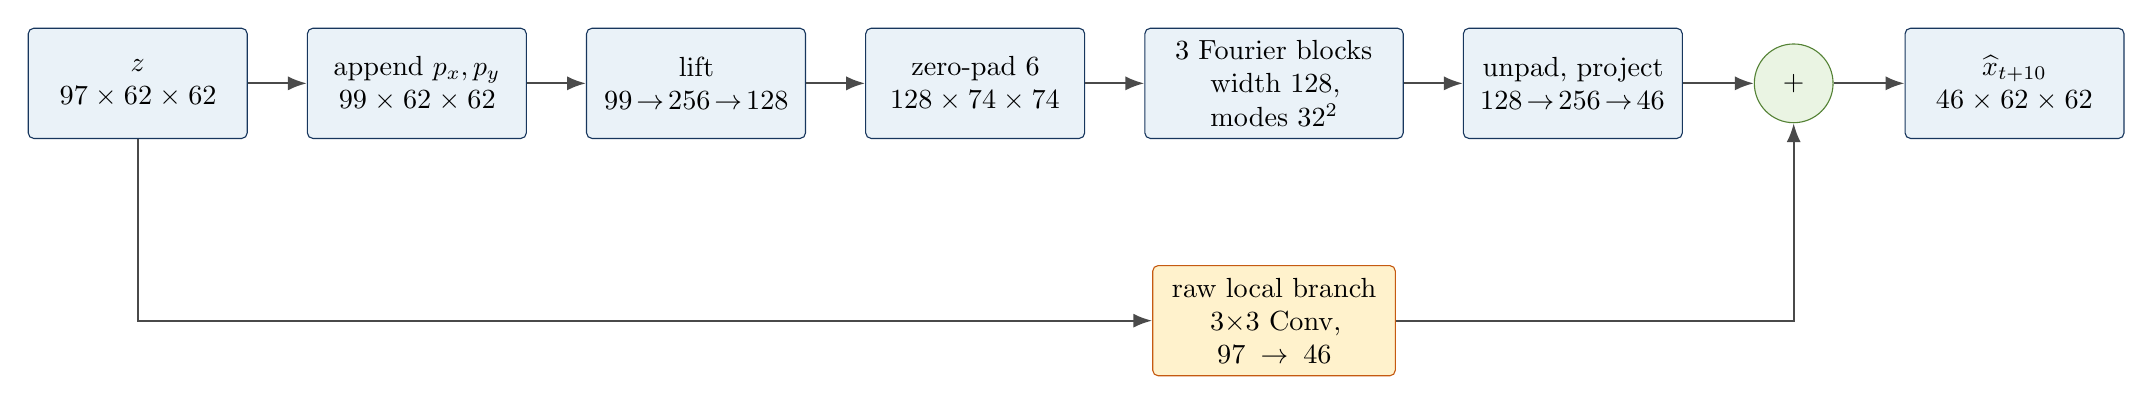
\begin{tikzpicture}[
  node distance=7.5mm,
  box/.style={
    draw=navy, fill=lightblue, rounded corners=2pt,
    minimum height=14mm, text width=25mm, align=center, inner sep=4pt
  },
  local/.style={
    draw=orange, fill=lightorange, rounded corners=2pt,
    minimum height=14mm, text width=28mm, align=center, inner sep=4pt
  },
  sum/.style={
    draw=green, fill=lightgreen, circle, minimum size=10mm, inner sep=0pt
  },
  arrow/.style={-{Latex[length=2.4mm]}, line width=0.8pt, color=graytext}
]
  \node[box] (input) {\(z\)\\\(97\times62\times62\)};
  \node[box, right=of input] (pos) {append \(p_x,p_y\)\\\(99\times62\times62\)};
  \node[box, right=of pos] (lift) {lift\\\(99\!\to\!256\!\to\!128\)};
  \node[box, right=of lift] (pad) {zero-pad 6\\\(128\times74\times74\)};
  \node[box, right=of pad, text width=30mm] (blocks) {3 Fourier blocks\\width 128, modes \(32^2\)};
  \node[box, right=of blocks] (proj) {unpad, project\\\(128\!\to\!256\!\to\!46\)};
  \node[sum, right=9mm of proj] (add) {\(+\)};
  \node[box, right=9mm of add] (output) {\(\widehat{x}_{t+10}\)\\\(46\times62\times62\)};
  \node[local, below=16mm of blocks] (conv) {raw local branch\\\(3{\times}3\) Conv, \(97\to46\)};
  \draw[arrow] (input) -- (pos);
  \draw[arrow] (pos) -- (lift);
  \draw[arrow] (lift) -- (pad);
  \draw[arrow] (pad) -- (blocks);
  \draw[arrow] (blocks) -- (proj);
  \draw[arrow] (proj) -- (add);
  \draw[arrow] (add) -- (output);
  \draw[arrow] (input.south) |- (conv.west);
  \draw[arrow] (conv.east) -| (add.south);
\end{tikzpicture}}
\caption{Exact global-plus-local network. Batch dimension is omitted. The
wet-mask multiplication is deliberately outside this module.}
\label{fig:architecture}
\end{figure}

\section{Deterministic position channels}

The custom position encoder appends one \(x\)-varying and one \(y\)-varying
field. For index \(j\) along an axis of length \(N\),
\begin{equation}
  p(j)=
  \begin{cases}
    \sin\!\left(\dfrac{\pi j}{2N}\right), & j\ \text{even},\\[4pt]
    \cos\!\left(\dfrac{\pi j}{2N}\right), & j\ \text{odd}.
  \end{cases}
\end{equation}
The coordinate buffers are deterministic and non-persistent; they have no
learned parameters. NeuralOperator's own positional embedding is explicitly
\code{null}, so coordinates are not appended twice.

\section{Global FNO path}

\subsection{Lift and pad}

A pointwise ChannelMLP lifts 99 channels as
\[
  99 \longrightarrow 256
  \xrightarrow{\mathrm{GELU}}
  128.
\]
Symmetric domain padding then adds six zero cells on every side:
\[
  62\times62 \longrightarrow 74\times74.
\]
The local branch is not padded this way.

\subsection{Three Fourier blocks}

There are three width-128 blocks. Each requests 32 Fourier modes in \(Y\) and
32 in \(X\). With a real FFT on the last axis, a dense complex spectral tensor
has stored shape
\[
  (128,128,32,17);
\]
the \(17\) is \(32/2+1\). The convolution is dense, unfactorized
(\code{factorization=null}), full precision, and has a 128-element real bias.

Let \(h_\ell\) be the input to block \(\ell\), \(K_\ell\) the spectral
convolution, \(W_\ell\) a learned bias-free \(1\times1\) skip, and \(g_\ell\) a
learned per-channel soft gate. Under pinned NeuralOperator 2.0.0 the exact
postactivation ordering is
\begin{align}
  a_\ell &=
    \operatorname{LN}_{2\ell}\!\left(K_\ell h_\ell\right)
    + W_\ell h_\ell, \label{eq:block1}\\
  \bar a_\ell &=
    \begin{cases}
      \operatorname{GELU}(a_\ell), & \ell<2,\\
      a_\ell, & \ell=2,
    \end{cases}\\
  b_\ell &= \operatorname{MLP}_\ell(\bar a_\ell)
    + g_\ell\odot h_\ell, \label{eq:block2}\\
  h_{\ell+1} &=
    \begin{cases}
      \operatorname{GELU}\!\left(\operatorname{LN}_{2\ell+1}(b_\ell)\right),
        & \ell<2,\\
      \operatorname{LN}_{2\ell+1}(b_\ell), & \ell=2.
    \end{cases}
\end{align}

\important{The first LayerNorm is applied to the spectral-convolution output
\emph{before} the linear FNO skip is added. Moving it after the sum changes the
implemented network even if the layer list looks similar.}

Each block MLP is
\[
  128 \longrightarrow 512
  \xrightarrow{\mathrm{GELU}}
  128,
\]
with biases and zero dropout. The six custom pointwise LayerNorms normalize the
128 channels independently at each spatial position, with
\(\eps=10^{-5}\). The final block omits the two outer GELUs shown above; its
internal ChannelMLP still contains its GELU.

\subsection{Unpad and project}

After block three, the six-cell border is removed and a pointwise projection
maps
\[
  128 \longrightarrow 256
  \xrightarrow{\mathrm{GELU}}
  46.
\]
There is no final activation.

\section{Local branch and final sum}

In parallel, a no-bias \(3\times3\) convolution with one-cell zero padding maps
the raw 97-channel input directly to 46 channels at \(62\times62\). Thus
\begin{equation}
  F_\theta(z)
  =
  F_{\mathrm{global}}([z,p_x,p_y])
  +
  \operatorname{Conv}^{97\rightarrow46}_{3\times3}(z).
\end{equation}
The constructor zeroes the local kernel for a fresh model. This experiment,
however, immediately performs a strict same-shape load from the trained
continuity parent, so the local branch in the actual run is not a zero
operator.

\important{A direct call to \code{model(features)} may be nonzero on land.
Wet masking occurs in the maintained training unroll and inference stepper
after the global/local sum. Any new inference API must apply the same mask.}

\section{Hyperparameters and parameter count}

\begin{table}[H]
\centering
\caption{Frozen architecture contract.}
\begin{tabularx}{\textwidth}{@{}lXlX@{}}
\toprule
Setting & Value & Setting & Value \\
\midrule
Grid & \(62\times62\) & Input/output & 97 / 46 \\
Position channels & 2 & Lift input & 99 \\
Hidden width & 128 & FNO blocks & 3 \\
Modes & \(32\times32\) & Padding fraction & 0.1 \\
Lift ratio & 2 & Projection ratio & 2 \\
ChannelMLP expansion & 4 & Dropout & 0 \\
Precision & full & Factorization & none \\
Pointwise LayerNorm & yes & Local kernel & \(3\times3\) \\
\bottomrule
\end{tabularx}
\end{table}

\begin{longtable}{@{}p{0.35\textwidth}p{0.27\textwidth}r@{}}
\caption{Exact trainable parameter accounting.}
\label{tab:params}\\
\toprule
Component & Tensor/transform & PyTorch elements \\
\midrule
\endfirsthead
\toprule
Component & Tensor/transform & PyTorch elements \\
\midrule
\endhead
Position encoding & deterministic buffers & 0 \\
Lift & \(99\to256\to128\) & 58,496 \\
Three spectral kernels & \(3\times(128,128,32,17)\), complex & 26,738,688 \\
Three spectral biases & \(3\times128\), real & 384 \\
Three FNO linear skips & bias-free \(1\times1\) & 49,152 \\
Three block ChannelMLPs & \(128\to512\to128\) & 395,136 \\
Three soft gates & one value per channel & 384 \\
Six pointwise LayerNorms & scale and shift & 1,536 \\
Projection & \(128\to256\to46\) & 44,846 \\
Local branch & \((46,97,3,3)\), no bias & 40,158 \\
\midrule
\textbf{Total} & complex tensors count as one element & \textbf{27,328,780} \\
\bottomrule
\end{longtable}

PyTorch counts a complex weight as one parameter element. If real and
imaginary parts are counted separately, the model represents 54,067,468 real
scalar degrees of freedom. The retained report records the PyTorch total,
27,328,780.

\chapter{Autoregressive state transition}
\label{ch:rollout}

\section{Six-call training unroll}

The dataset returns two observed initial states and six truth targets:
\[
  \left(x_{t-10},x_t;
  x_{t+10},x_{t+20},\ldots,x_{t+60}\right).
\]
The maintained \repo{two_in_state_unroll} performs:
\begin{align*}
  \widehat{x}_{t+10} &= F(x_{t-10},x_t,s),\\
  \widehat{x}_{t+20} &= F(x_t,\widehat{x}_{t+10},s),\\
  \widehat{x}_{t+30} &= F(\widehat{x}_{t+10},
                              \widehat{x}_{t+20},s),\\
  &\ \vdots\\
  \widehat{x}_{t+60} &= F(\widehat{x}_{t+40},
                              \widehat{x}_{t+50},s).
\end{align*}
After every call, all 46 output channels are multiplied by the broadcast wet
mask. The output tensor has shape \((N,6,46,62,62)\). There is no teacher
forcing after the two initial observed states, and the five statics remain
fixed.

\begin{lstlisting}
previous = observed_at_t_minus_10
current = observed_at_t
predictions = []
for call in range(number_of_calls):
    features = concat(previous, current, fixed_statics)
    future = model(features) * wet_mask
    predictions.append(future)
    previous, current = current, future
\end{lstlisting}

\section{Long inference}

\repo{BireTwoInNewChannelsStepper.step} implements the same two-state shift and
static-channel construction for inference. The maintained held evaluation
calls it 200 times to reach day 2000. When building a new inference consumer,
load the exact architecture and normalization declared by the checkpoint,
supply two consecutive normalized initial states, keep the static block
unchanged, and apply the wet mask at every step.

\section{Shape assertions worth preserving}

\begin{itemize}
  \item Features: \((N,97,62,62)\), NCHW, float tensor.
  \item Position-augmented lift input: \((N,99,62,62)\).
  \item One-step output: \((N,46,62,62)\).
  \item Training rollout: \((N,6,46,62,62)\).
  \item Wet mask passed to rollout: broadcastable from \((1,1,62,62)\).
  \item Physical static block before batch selection: \((3,5,62,62)\).
\end{itemize}

\chapter{Complete training objective}
\label{ch:loss}

\section{Total objective}

The final loss is
\begin{align}
L={}&L_{\mathrm{state}}
+10^{-3}L_{\mathrm{increment}}
+0.50L_{\mathrm{rollout}}
+10^{-5}L_{\mathrm{spectral}}
+0.065L_{\mathrm{boundary}}
\nonumber\\
&+0.05L_{\mathrm{pressure}}
+0.05L_{\mathrm{continuity}}
+0.05L_{\mathrm{BT}}.
\label{eq:total-loss}
\end{align}
The first five terms are implemented in \repo{objective.py} and orchestrated by
\repo{_train_core.py}. The final wrapper in \repo{train.py} captures that base
loss and adds the three physics terms.

For a prediction \(a\), target \(b\), and mask \(M\), the recurring
truth-normalized form is
\begin{equation}
  r(a,b;M)
  =
  \left(
    \frac{\sum M(a-b)^2}
         {\max(\sum Mb^2,\eps)}
  \right)^{1/2}.
\end{equation}
Some auxiliary terms intentionally use the squared ratio without the square
root; those cases are identified below.

\section{Five inherited emulator terms}

\begin{description}
  \item[State, \(L_{\mathrm{state}}\).]
  Masked relative \(\Ltwo\) at the first forecast, day 10. U, V, temperature,
  and surface height each receive one quarter of the group mean, preventing the
  15-level fields from overwhelming the single surface-height channel.

  \item[Increment, \(L_{\mathrm{increment}}\).]
  At day 10, compare
  \((\widehat{x}_{t+10}-x_t)\) with
  \((x_{t+10}-x_t)\). Compute a group-balanced RMSE after dividing each channel
  by its inherited training-only increment scale.

  \item[Rollout, \(L_{\mathrm{rollout}}\).]
  Group-balanced state relative \(\Ltwo\), averaged over calls 2--6
  (days 20--60). Day 10 is already covered by the state term.

  \item[Spectral, \(L_{\mathrm{spectral}}\).]
  For each of the six chained ten-day increments, crop the exact wet rectangle,
  spatially demean, apply a two-dimensional Hann taper, compute an orthonormal
  real FFT, and compare radial amplitudes in 12 bins. Average equally over the
  four state groups and all calls.

  \item[Western boundary, \(L_{\mathrm{boundary}}\).]
  State relative \(\Ltwo\) on the first four wet cells east of the western wall,
  averaged over all six calls. The mask comes from the dataset's
  boundary-index construction.
\end{description}

\section{Pressure-gradient term}

The pressure term first de-normalizes all predictions and targets. It
reconstructs 15 levels of total hydrostatic potential
\(\Phi_{\mathrm{hyd}}\) from \(\Theta\) and \(\eta\), using
\[
  g=9.81\ \mathrm{m\,s^{-2}},
  \qquad
  \alpha=2.0\times10^{-4}\ \mathrm{K^{-1}},
\]
the exact layer thicknesses
\[
  \Delta r=(50,60,70,80,90,100,110,120,130,140,150,160,170,180,190)
  \ \mathrm{m},
\]
and reference temperatures
\[
  T_{\mathrm{ref}}=(30,27,24,21,18,15,13,11,9,7,6,5,4,3,2)^\circ\mathrm{C}.
\]
The active recurrence integrates the linear-EOS density anomaly
\(-\alpha(\Theta-T_{\mathrm{ref}})\) between interfaces and cell centers, then
adds \(g\eta\) to every level.

Neighboring tracer-point differences place the pressure gradients on C-grid
velocity faces:
\begin{align}
  G_x &= \frac{\Phi_{i,j+1}-\Phi_{i,j}}
              {\tfrac12(DXF_{i,j+1}+DXF_{i,j})},\\
  G_y &= \frac{\Phi_{i+1,j}-\Phi_{i,j}}
              {R_{\mathrm E}\,\pi/180},
  \qquad R_{\mathrm E}=6.370\times10^6\ \mathrm m.
\end{align}
Only faces whose two tracer cells are wet contribute. The loss is the rooted
truth-relative \(\Ltwo\), averaged equally over \(x/y\), 15 levels, batches, and
six rollout calls. A uniform offset in \(\eta\) is dynamically invisible
because its horizontal gradient is zero.

\section{Free-surface continuity term}

Depth-integrated transports in physical units are
\begin{equation}
  Q_x(x)=\sum_{k=1}^{15}U_k(x)\Delta r_k,
  \qquad
  Q_y(x)=\sum_{k=1}^{15}V_k(x)\Delta r_k.
\end{equation}
For a ten-day pair \((a,b)\), the implemented truth-referenced residual is
\begin{equation}
  R(a,b)
  =
  \frac{\eta_b-\eta_a}{864000}
  +
  \nabla\cdot
  \left[\frac{Q(a)+Q(b)}{2}\right].
\end{equation}
The divergence uses centered tracer-point differences, local \code{DXF} in
\(x\), one Earth-degree in \(y\), and only interior locations whose complete
five-point stencil is wet.

The first predicted residual is \(R(x_t,\widehat{x}_{t+10})\); later residuals
chain from the preceding prediction. Truth residuals chain truth-to-truth.
For each call, the implementation uses
\begin{equation}
  \frac{\|R_{\mathrm{pred}}-R_{\mathrm{truth}}\|_2^2}
       {\|R_{\mathrm{truth}}\|_2^2+\eps},
\end{equation}
then averages over batch and calls. There is deliberately no square root.
The target is the truth residual rather than zero because ten-day samples and
centered U/V fields only approximate MITgcm's native discrete operator.

\section{Barotropic-transport increment term}

The new term reuses \(Q_x,Q_y\), takes no horizontal derivative, and compares
successive finite transport increments:
\begin{equation}
  \Delta Q^{p}_{s,\mathrm{pred}}
    =Q^{p}(\widehat{x}_{s})-Q^{p}(\widehat{x}_{s-1}),
  \qquad p\in\{x,y\},
\end{equation}
where the observed present \(x_t\) is the predecessor for call one. Truth
increments are always truth-to-truth. The wet-masked objective is
\begin{equation}
  L_{\mathrm{BT}}
  =
  \frac{1}{6}\sum_{s=1}^{6}\frac12
  \left[
    \frac{\|\Delta Q^x_{s,\mathrm{pred}}
              -\Delta Q^x_{s,\mathrm{truth}}\|_2^2}
         {\|\Delta Q^x_{s,\mathrm{truth}}\|_2^2+\eps}
    +
    \frac{\|\Delta Q^y_{s,\mathrm{pred}}
              -\Delta Q^y_{s,\mathrm{truth}}\|_2^2}
         {\|\Delta Q^y_{s,\mathrm{truth}}\|_2^2+\eps}
  \right].
\end{equation}
Zonal and meridional components receive exactly equal weight. Only U/V
channels receive gradients from this term.

\important{The contract calls this a ten-day tendency, but the code uses
the finite increment and does not divide by 864000 s. The missing common
factor cancels from each relative ratio, so the numerical loss is equivalent;
call it an increment when describing the implementation.}

\chapter{Training and checkpoint production}
\label{ch:training}

\section{Specialized wrapper over a shared engine}

\repo{oceanfno.train} is not an independent training loop. Its
\code{run()} routine builds pressure, continuity, and barotropic contexts;
captures the base loss; monkey-patches selected functions and constants in
\repo{oceanfno._train_core}; and delegates to the shared engine.

\important{Changing only \repo{_train_core.model_c_loss_terms} does not
necessarily change this model's effective loss: \repo{train.py} replaces it
with \code{_loss_with_physics_terms}. Trace the wrapper and shared engine
together before editing training behavior.}

The high-level execution is:
\begin{enumerate}
  \item parse and validate the frozen target contract;
  \item verify source paths and SHA-256 hashes;
  \item build the 97-input architecture;
  \item strict-load only the parent's model state;
  \item reuse parent normalization and increment scales;
  \item create a new Adam optimizer with no inherited moments;
  \item train for 3,840 new updates, staging all outputs;
  \item evaluate four saved checkpoints;
  \item select one checkpoint, write reports/arrays/manifest, then atomically
        publish the staging directories.
\end{enumerate}

\section{Optimizer and schedule}

\begin{table}[H]
\centering
\caption{Effective fine-tuning schedule.}
\begin{tabularx}{\textwidth}{@{}lXlX@{}}
\toprule
Setting & Value & Setting & Value \\
\midrule
Optimizer & Adam, freshly initialized & Batch size & 4 \\
Betas & \((0.9,0.95)\) & Weight decay & 0 \\
Initial learning rate & \(2\times10^{-5}\) & Gradient clipping & none \\
Decay point & after step 2880 & Decay factor & 0.2 \\
Final learning rate & \(4\times10^{-6}\) & Maximum step & 3840 \\
Checkpoints & 960, 1920, 2880, 3840 & Seed & 20260724 \\
Rollout calls/update & 6 & Parent optimizer & not loaded \\
\bottomrule
\end{tabularx}
\end{table}

The DataLoader uses \code{ChunkAwareBatchSampler}, \code{num_workers=0}, and
pinned host memory on CUDA. A batch never crosses regime boundaries.

\section{Initialization and checkpoint semantics}

The pinned parent selected checkpoint is:
\begin{lstlisting}
/bigscratch/mjalabert314/bire_james25_repro/af_fno/models/C/
  model_c_2in_1out_new_channels_pressure_gradient_continuity_v1/selected.pt

SHA-256:
bd25ad0b09412a3865896df3dafe4f14bc838cedbef914792a059354af0e3986
\end{lstlisting}

The load is strict and same-shape, so it is function-preserving at step zero.
Only \code{model_state_dict} is loaded. Checkpoints produced by the final
fine-tune contain model state and provenance metadata but no optimizer state.
Consequently there is no exact Adam-resume path; restarting from a saved model
creates a new optimization trajectory.

\section{Output transaction and overwrite protection}

The engine writes to staging directories ending in \code{.tmp}, completes all
validation/publication work, and atomically renames them. It stops if either
the final or staging project/scratch directory already exists. This protects
retained evidence but means a scheduler retry cannot simply reuse the same
contract after partial output. Inspect and move a failed staging directory, or
choose a fresh versioned output; never delete it without first determining
whether it contains the only checkpoint copy.

\section{Retained training result}

\begin{table}[H]
\centering
\caption{Published training result.}
\begin{tabularx}{\textwidth}{@{}lX@{}}
\toprule
Item & Retained value \\
\midrule
Status & complete \\
Selected fine-tune step & 3840; only feasible checkpoint \\
Parameter count & 27,328,780 \\
Training records & 17,790 \\
Slurm job / elapsed & 331057 / 7,708.5 s (about 2 h 8 min) \\
Selected checkpoint SHA-256 &
\code{bf3ccc704ff12cc4b7354bddc21e858ad}\newline
\code{96c0214ba9c86d02c1510b52ff9ff52} \\
\bottomrule
\end{tabularx}
\end{table}

\begin{figure}[H]
\centering
\safegraphic[width=0.90\textwidth]{../outputs/af_fno/C/model_c_2in_1out_new_channels_p_cont_BT_loss/model_c_2in_1out_new_channels_p_cont_BT_loss_v1/model_c_2in_1out_new_channels_p_cont_BT_loss_selection.png}
\caption{Retained checkpoint-selection figure. The report, not the PNG alone,
is the authoritative numerical record.}
\label{fig:selection}
\end{figure}

\chapter{Validation and model selection}
\label{ch:validation}

\section{Validation rollouts}

Each of the four checkpoints is evaluated on 102 autonomous 360-day rollouts:
34 starts per regime, at 6000, 6006, \ldots, 6198. The model is scored every
ten days against:

\begin{itemize}
  \item truth,
  \item persistence from the present state, and
  \item a train-only, regime-specific climatology.
\end{itemize}

Primary RMSE fields are surface speed, SST, and surface
\(\Phi_{\mathrm{hyd}}\). ACC through day 200 is computed for surface U,
surface V, SST, and surface \(\Phi_{\mathrm{hyd}}\). Diagnostics also include
maximum normalized magnitude and day-360 biases.

\section{Selection rule}

For each primary field, compute its checkpoint-wise 10--90-day RMSE AUC. A
checkpoint is feasible only if all three short AUCs are at most 1.05 times
their respective best checkpoint values. Among feasible checkpoints, minimize
the worst 90--360-day RMSE-AUC ratio to climatology; ties go to the earlier
checkpoint. Only step 3840 was feasible.

\begin{table}[H]
\centering
\caption{Selected step-3840 validation metrics.}
\begin{tabular}{@{}lrrr@{}}
\toprule
Metric & Surface speed & SST & Surface \(\Phi_{\mathrm{hyd}}\) \\
\midrule
Short AUC, days 10--90 & 0.08299065 & 0.90202660 & 0.29725232 \\
Short AUC / parent & 0.967303 & 0.984124 & 0.980390 \\
Long AUC / climatology, days 90--360 & 0.377685 & 0.478730 & 0.128824 \\
\bottomrule
\end{tabular}
\end{table}

Day-200 ACC was 0.956278 for U, 0.935325 for V, 0.906777 for SST, and
0.993512 for surface \(\Phi_{\mathrm{hyd}}\). The validation acceptance gate
passed: short skill was not more than five percent worse than the parent, the
worst long ratio was below 0.85, and it did not regress from the parent.

\section{What validation does not establish}

The validation horizon is 360 days and pools all three regimes. It does not
guarantee day-2000 skill, it does not provide a disjoint inference split, and it
does not test a changed grid or forcing family. Long S0 behavior must be read
from the held figure package described next.

\chapter{Held inference, figures, and anomaly postprocessing}
\label{ch:inference}

\section{Maintained inference entry point}

There is no standalone general-purpose inference command. The maintained
checkpoint loading and held rollout are executed by:
\begin{lstlisting}
./.venv/bin/python -m oceanfno.figures finalize \
  --contract config/model_c_2in_1out_new_channels_p_cont_BT_loss_s0_figures_v1.json

./.venv/bin/python -m oceanfno.figures preflight \
  --contract config/model_c_2in_1out_new_channels_p_cont_BT_loss_s0_figures_v1.json

./.venv/bin/python -m oceanfno.figures run \
  --contract config/model_c_2in_1out_new_channels_p_cont_BT_loss_s0_figures_v1.json \
  --device cuda
\end{lstlisting}

\code{finalize} fills only allowed pending provenance fields and writes the JSON
in place. \code{preflight} verifies every pinned source. \code{run}
strict-loads the model, constructs the canonical stepper, rolls it out, computes
metrics, plots, and publishes a sealed package.

\section{S0 protocol}

The deterministic seed 20260802 selects these 15 S0 starts:
\begin{lstlisting}
6263, 6293, 6331, 6389, 6579,
6593, 6598, 6601, 6651, 6661,
6694, 6707, 6711, 6968, 6979
\end{lstlisting}

Each member receives truth at \(t-10\) and \(t\). The final selected model runs
200 autonomous calls to day 2000. The continuity-parent comparator runs only
to day 200 for ACC. Both use the selected model's reused normalization and
the same five-static architecture.

\begin{table}[H]
\centering
\caption{Canonical figure products.}
\begin{tabularx}{\textwidth}{@{}lX@{}}
\toprule
Product & Content \\
\midrule
Figure 3 & Member-0 transport streamfunction, days 0, 10, 20, 30, 40 \\
Figure 4 & Ensemble RMSE through day 200 \\
Figure 5 & Member-0 RMSE \\
Figure 6 & Selected versus continuity-parent ACC through day 200 \\
Figure 7 & Member-0 streamfunction at days 60 and 2000 \\
Figure 8 & Ensemble RMSE through day 2000 \\
Machine-readable & CSV curves, compressed NPZ arrays, JSON summary/report,
manifest, and acceptance-gate JSON \\
\bottomrule
\end{tabularx}
\end{table}

\begin{figure}[H]
\centering
\safegraphic[height=0.76\textheight,keepaspectratio]{../outputs/af_fno/C/model_c_2in_1out_new_channels_p_cont_BT_loss/model_c_2in_1out_new_channels_p_cont_BT_loss_s0_figures_v1/S0/model_c_bire_figure6_dt10_acc_0_200_days_s0.png}
\caption{Retained selected-versus-parent ACC comparison. The comparison is a
literal loss fine-tune pair with identical architecture.}
\label{fig:acc}
\end{figure}

\begin{figure}[H]
\centering
\safegraphic[height=0.76\textheight,keepaspectratio]{../outputs/af_fno/C/model_c_2in_1out_new_channels_p_cont_BT_loss/model_c_2in_1out_new_channels_p_cont_BT_loss_s0_figures_v1/S0/model_c_bire_figure8_dt10_rmse_0_2000_days_s0.png}
\caption{Retained ensemble RMSE through day 2000.}
\label{fig:longrmse}
\end{figure}

\section{Held results and interpretation}

The inference job was Slurm job 331312 and took 66.12 s. At day 200 the
selected model's ACC exceeded the parent for every plotted field:

\begin{table}[H]
\centering
\caption{Day-200 ACC on the held S0 members.}
\begin{tabular}{@{}lrr@{}}
\toprule
Field & Continuity parent & BT-loss fine-tune \\
\midrule
Surface U & 0.918266 & 0.924516 \\
Surface V & 0.948361 & 0.950639 \\
SST & 0.911161 & 0.916013 \\
Surface \(\Phi_{\mathrm{hyd}}\) & 0.996434 & 0.996633 \\
\bottomrule
\end{tabular}
\end{table}

\begin{table}[H]
\centering
\caption{Mean day-2000 RMSE.}
\begin{tabular}{@{}lrrr@{}}
\toprule
Field & Model & Persistence & Climatology \\
\midrule
Surface speed & 0.0055045 & 0.0051005 & 0.0035868 \\
SST & 0.0591130 & 0.0595483 & 0.0404577 \\
Surface \(\Phi_{\mathrm{hyd}}\) & 0.0278762 & 0.0382424 & 0.0824887 \\
\bottomrule
\end{tabular}
\end{table}

The automated measurable gate passed: outputs were finite; maximum normalized
magnitude was 6.70786 against a limit of 8; member-0 day-2000 streamfunction
minimum was \(-30.2363\) Sv against a lower limit of \(-33\) Sv; and its
spatial-standard-deviation ratio to truth was 0.997956 within
\([0.8,1.25]\).

\important{A gate pass is not uniform long-horizon superiority. The day-2000
RMSE/climatology ratios were 0.338 for surface
\(\Phi_{\mathrm{hyd}}\), 1.461 for SST, and 1.535 for surface speed. The model
beats climatology strongly for pressure but is worse for SST and speed at that
lead. The gate also retains a manual visual check for western-boundary
sharpness, recognizable gyre structure, and basin-wide smoothing.}

\section{Anomaly postprocessing}

The anomaly command is:
\begin{lstlisting}
./.venv/bin/python -m oceanfno.anomaly finalize \
  --contract config/model_c_2in_1out_new_channels_p_cont_BT_loss_s0_anomaly_v1.json

./.venv/bin/python -m oceanfno.anomaly preflight \
  --contract config/model_c_2in_1out_new_channels_p_cont_BT_loss_s0_anomaly_v1.json

./.venv/bin/python -m oceanfno.anomaly run \
  --contract config/model_c_2in_1out_new_channels_p_cont_BT_loss_s0_anomaly_v1.json
\end{lstlisting}

This stage does not load a checkpoint and does not rerun inference. It reads
the sealed figure arrays, computes the S0 MITgcm mean streamfunction over
training days 0--5999, subtracts that same mean field from model and truth, and
publishes Figure 3a, Figure 7a, a mean-reference plot, arrays, report, and
manifest.

The retained job 331353 took 26.1 s. At day 2000 the model anomaly RMS was
0.46384 Sv versus 0.19449 Sv for truth, a ratio of 2.38493; the western
four-cell RMS ratio was 1.5707.

\begin{figure}[H]
\centering
\safegraphic[width=0.94\textwidth]{../outputs/af_fno/C/model_c_2in_1out_new_channels_p_cont_BT_loss/model_c_2in_1out_new_channels_p_cont_BT_loss_s0_anomaly_v1/S0/model_c_bire_figure7a_streamfunction_anomaly_day060_day2000_s0.png}
\caption{Retained streamfunction-anomaly comparison at days 60 and 2000.}
\label{fig:anomaly}
\end{figure}

\chapter{Configuration contracts and artifact provenance}
\label{ch:contracts}

\section{Three active forward contracts}

\begin{longtable}{@{}p{0.31\textwidth}p{0.23\textwidth}p{0.38\textwidth}@{}}
\caption{Active configuration files for this model.}
\label{tab:contracts}\\
\toprule
Contract & Entry point & Responsibility \\
\midrule
\endfirsthead
\toprule
Contract & Entry point & Responsibility \\
\midrule
\endhead
\repo{config/model_c_2in_1out_new_channels_p_cont_BT_loss_v1.json} &
\code{oceanfno.train} &
Architecture, parent initialization, all physics-loss declarations, source
hashes, output roots, and optimizer schedule. \\
\repo{config/model_c_2in_1out_new_channels_p_cont_BT_loss_s0_figures_v1.json} &
\code{oceanfno.figures} &
Selected/comparator identities, identical architectures, normalization,
dataset/MITgcm sources, S0 member protocol, and figure output roots. \\
\repo{config/model_c_2in_1out_new_channels_p_cont_BT_loss_s0_anomaly_v1.json} &
\code{oceanfno.anomaly} &
Sealed figure arrays/report/manifest, S0 training-mean definition, output
names, and CPU postprocessing roots. \\
\bottomrule
\end{longtable}

The training contract is fully materialized; there is no generic
\code{inherit_parent_fields}. Inheritance is semantic and enforced by the
strict parent checkpoint plus reused parent normalization/report.

\section{What preflight protects}

Training preflight checks contract semantics and hashes for the Zarr metadata,
parent checkpoint, parent normalization, parent report, MITgcm declaration,
SST relaxation binary, and DXF binary. Figure preflight additionally verifies
the selected report/checkpoint/normalization and comparator. Anomaly preflight
verifies the sealed figure contract, manifest, report, arrays, and dataset
metadata.

The downstream \code{finalize} commands are controlled mutations: they fill
pending upstream-derived fields and their digests, reject conflicting sealed
values, and rewrite the JSON. Run them only in a writable working tree and
review the diff.

\section{Retained artifact layout}

The lightweight project package contains reports, arrays, plots, README files,
and manifests. Large checkpoints and selected model files live in scratch.
The current grouped project layout is:
\begin{lstlisting}
outputs/af_fno/C/model_c_2in_1out_new_channels_p_cont_BT_loss/
  model_c_2in_1out_new_channels_p_cont_BT_loss_v1/
  model_c_2in_1out_new_channels_p_cont_BT_loss_s0_figures_v1/
    S0/
  model_c_2in_1out_new_channels_p_cont_BT_loss_s0_anomaly_v1/
    S0/
\end{lstlisting}

The scratch training directory contains four approximately 216 MB checkpoints,
\code{selected.pt}, reused normalization, arrays, and the report. Reports,
arrays, checkpoints, and scheduler logs are ignored by Git; only selected PNGs
are generally tracked. A clean clone therefore needs access to the shared
scratch artifacts to reproduce provenance.

\section{Known stale generated text}

Two retained prose notes are not authoritative:

\begin{itemize}
  \item the figure-package README says the comparator and selected model use
        different static channels; active \repo{figures.py} and the figure
        contract show identical physical-static architectures;
  \item a nested training-report note says the warm start is not
        function-preserving; the contract and active \repo{train.py} enforce a
        strict same-shape load, and measured perturbation at load is zero.
\end{itemize}

Use machine fields plus active code, not those inherited sentences.

\chapter{Slurm and cluster runbook}
\label{ch:slurm}

\section{Resource requests}

\begin{table}[H]
\centering
\caption{Resources declared by the maintained launchers.}
\begin{tabularx}{\textwidth}{@{}lXXXXXX@{}}
\toprule
Stage & Partition & GPU & CPUs & Memory & Time & Modules \\
\midrule
Training & \code{gpu} & 1 V100 & 4 & default & 5 h &
GNU 12.2, CUDA 12.4 \\
Figures/inference & \code{gpu} & 1 V100 & 4 & default & 1 h &
GNU 12.2, CUDA 12.4 \\
Anomaly & \code{batch} & none & 4 & 16 GB & 30 min &
GNU 12.2 \\
\bottomrule
\end{tabularx}
\end{table}

All jobs use account \code{pod-users}, one node, and one task. GPU launchers
set OMP/MKL threads to four and print \code{nvidia-smi}. The scripts do not set
explicit \code{--output} or \code{--error}, so normal Slurm log naming applies.

\section{Direct commands}

Training:
\begin{lstlisting}
./.venv/bin/python -m oceanfno.train preflight \
  --contract config/model_c_2in_1out_new_channels_p_cont_BT_loss_v1.json

./.venv/bin/python -m oceanfno.train run \
  --contract config/model_c_2in_1out_new_channels_p_cont_BT_loss_v1.json \
  --device cuda
\end{lstlisting}

Figures/inference:
\begin{lstlisting}
./.venv/bin/python -m oceanfno.figures finalize \
  --contract config/model_c_2in_1out_new_channels_p_cont_BT_loss_s0_figures_v1.json
./.venv/bin/python -m oceanfno.figures preflight \
  --contract config/model_c_2in_1out_new_channels_p_cont_BT_loss_s0_figures_v1.json
./.venv/bin/python -m oceanfno.figures run \
  --contract config/model_c_2in_1out_new_channels_p_cont_BT_loss_s0_figures_v1.json \
  --device cuda
\end{lstlisting}

Anomaly:
\begin{lstlisting}
./.venv/bin/python -m oceanfno.anomaly finalize \
  --contract config/model_c_2in_1out_new_channels_p_cont_BT_loss_s0_anomaly_v1.json
./.venv/bin/python -m oceanfno.anomaly preflight \
  --contract config/model_c_2in_1out_new_channels_p_cont_BT_loss_s0_anomaly_v1.json
./.venv/bin/python -m oceanfno.anomaly run \
  --contract config/model_c_2in_1out_new_channels_p_cont_BT_loss_s0_anomaly_v1.json
\end{lstlisting}

\section{Safe new-run checklist}

\begin{enumerate}
  \item Create a descriptive new version; never reuse an output version whose
        project or scratch directory exists.
  \item Copy, rename, and review the training contract. Change
        \code{version}, \code{output.project_root}, and
        \code{output.scratch_root}; preserve source hashes unless the source is
        intentionally changed.
  \item Run training preflight locally. Save its JSON output with the run
        record.
  \item Submit training and wait for a complete report, selected checkpoint,
        normalization, and manifest.
  \item Copy the figure contract, point it at the new selected report,
        checkpoint, and normalization, set only the wrapper-supported
        upstream-derived fields to pending, then run \code{finalize}.
  \item Review the finalized JSON diff and run figure preflight before
        submission.
  \item Repeat the copy/finalize/preflight sequence for anomaly
        postprocessing.
  \item Verify all manifest hashes and archive scheduler job IDs, elapsed time,
        environment versions, contract digests, and selected checkpoint hash.
\end{enumerate}

\section{Failure triage}

\begin{description}
  \item[Pinned source changed.]
  Resolve the exact path and calculate which artifact the contract intended.
  A relocation can cause this even when contents are intact. Do not edit only
  the hash.

  \item[Output already exists.]
  The transaction guard is working. Inspect both final and \code{.tmp}
  directories. Choose a new version unless an incomplete staging directory is
  intentionally recovered.

  \item[CUDA or NeuralOperator mismatch.]
  Confirm the job loaded CUDA 12.4, the interpreter is the repository
  \repo{.venv/bin/python}, Torch reports CUDA support, and NeuralOperator is
  exactly 2.0.0.

  \item[Land values are nonzero.]
  Check whether the caller used the maintained unroll/stepper. The network
  module itself does not mask land.

  \item[Unexpected loss change.]
  Inspect \repo{train.py}'s installed patches in addition to
  \repo{_train_core.py}. Print the returned loss-term dictionary in a small
  CPU test before a GPU submission.
\end{description}

\chapter{Tests and current verification status}
\label{ch:tests}

\section{Focused forward test command}

\begin{lstlisting}
PYTHONDONTWRITEBYTECODE=1 .venv/bin/python -m pytest \
  -p no:cacheprovider -q \
  tests/test_train.py tests/test_figures.py tests/test_anomaly.py
\end{lstlisting}

On 14 August 2026 the result was:
\begin{lstlisting}
3 failed, 25 passed
\end{lstlisting}

All three failures are \code{FileNotFoundError} in the lineage assertions at the
start of \repo{tests/test_train.py}. They try to read two absent active
contracts:
\begin{lstlisting}
config/model_c_2in_1out_new_channels_pressure_gradient_continuity_v1.json
config/model_c_2in_1out_new_channels_v1.json
\end{lstlisting}
The failed assertions were intended to prove unchanged architecture and
loss-only succession. Because this handbook deliberately does not use
\repo{archive/}, the current focused suite cannot honestly be described as
green until those active lineage fixtures are restored or the tests are made
self-contained.

\section{What the passing tests cover}

\begin{longtable}{@{}p{0.23\textwidth}p{0.69\textwidth}@{}}
\caption{Forward test coverage.}
\label{tab:tests}\\
\toprule
File & Covered behavior \\
\midrule
\endfirsthead
\toprule
File & Covered behavior \\
\midrule
\endhead
\repo{tests/test_train.py} &
Target contract loading without cluster-source verification; parent
checkpoint identity; canonical Slurm entry point; PHIHYD shape, identity,
uniform-offset invariance, temperature/SSH gradients; exact MITgcm layer
thicknesses; continuity identity, chaining, divergence-free uniform transport,
and gradients; barotropic identity, increment semantics, equal zonal/meridional
weight, and velocity-only gradients. \\
\repo{tests/test_figures.py} &
Same architecture for selected and comparator; retained continuity-parent
identity; pending-or-sealed digest rules; deterministic inference bounds; and
canonical figure Slurm entry point. \\
\repo{tests/test_anomaly.py} &
No checkpoint dependency; sealed figure-array inputs; fixed scientific
protocol; digest state; and canonical anomaly Slurm entry point. \\
\bottomrule
\end{longtable}

\section{Coverage gaps}

The focused tests do not execute the full optimizer, exact checkpoint reload
and selection, 360-day validation, 2,000-day inference, plotting, atomic
publication, manifest sealing, or overwrite guards end to end. Before a
scientific release, add at least one small synthetic smoke contract that runs
the complete pipeline on CPU, plus a cluster preflight against the real pinned
sources.

\section{Minimum tests after common edits}

\begin{table}[H]
\centering
\caption{Recommended verification by change type.}
\begin{tabularx}{\textwidth}{@{}lX@{}}
\toprule
Change & Required checks \\
\midrule
Channel order or normalization &
Dataset shape/unit test, round-trip de-normalization, physics-context test,
checkpoint compatibility failure test, and inference-stepper test. \\
FNO width/modes/layers &
Architecture-contract equality, exact parameter count, forward/backward shape,
checkpoint load behavior, and a short autonomous stability rollout. \\
New loss term &
Identity-zero test, deliberately perturbed nonzero test, channel-gradient
support test, component weighting test, and six-call chaining test. \\
Training schedule &
Contract validation, actual learning-rate trace, checkpoint step list,
selection input list, and no-resume semantics. \\
Figure protocol &
Deterministic starts, lead grid, sealed hashes, comparator identity, array
schema, and plot smoke test. \\
\bottomrule
\end{tabularx}
\end{table}

\chapter{Code architecture and maintenance guide}
\label{ch:maintenance}

\section{Active module map}

\begin{longtable}{@{}p{0.31\textwidth}p{0.61\textwidth}@{}}
\caption{Forward code ownership.}
\label{tab:modules}\\
\toprule
Module & Responsibility \\
\midrule
\endfirsthead
\toprule
Module & Responsibility \\
\midrule
\endhead
\repo{src/oceanfno/runtime.py} &
Lazy dependency imports/version checks, canonical channel names, hashing and
runtime helpers, chunk-aware batching. \\
\repo{src/oceanfno/dataset.py} &
Bire temporal windows, Zarr access, pointwise normalization, five-static
construction, training dataset, boundary masks. \\
\repo{src/oceanfno/model.py} &
Architecture dataclasses, deterministic position encoding, pointwise
LayerNorm, FNO builder, global/local model, training unroll, inference
steppers. \\
\repo{src/oceanfno/objective.py} &
Group-balanced state, increment, rollout, spectral, and western-boundary
objectives. \\
\repo{src/oceanfno/pressure_gradient.py} &
Differentiable PHIHYD reconstruction and face-gradient loss. \\
\repo{src/oceanfno/continuity.py} &
Physical depth integration, centered transport divergence, chained
truth-referenced continuity loss. \\
\repo{src/oceanfno/barotropic_transport.py} &
Depth-integrated zonal/meridional transport-increment loss. \\
\repo{src/oceanfno/_train_core.py} &
Reusable dataset/optimizer loop, checkpoint writing, validation, selection,
publication, and report generation. \\
\repo{src/oceanfno/train.py} &
Final-model contract validation, parent loading, physics contexts, monkey
patches, CLI specialization. \\
\repo{src/oceanfno/validation.py} &
360-day rollout metrics, AUCs, feasibility rule, selected-step decision. \\
\repo{src/oceanfno/diagnostics.py} &
Physical derived fields including PHIHYD, surface speed, and streamfunction. \\
\repo{src/oceanfno/_figures_core.py} &
Deterministic S0 member sampling, 2,000-day rollout, metrics, arrays,
acceptance gate, and atomic publication. \\
\repo{src/oceanfno/figures.py} &
Final-model/comparator contract wrapper, source verification, strict model
loading, CLI specialization. \\
\repo{src/oceanfno/plots.py} &
Canonical Figure 3--8 filenames and plot construction. \\
\repo{src/oceanfno/_anomaly_core.py} &
Training-mean streamfunction reference, anomaly arrays/figures, atomic
publication. \\
\repo{src/oceanfno/anomaly.py} &
Sealed-input verification and anomaly CLI specialization. \\
\bottomrule
\end{longtable}

\section{Safe modification recipes}

\subsection{Changing the architecture}

\begin{enumerate}
  \item Add a new version rather than editing the frozen final contract.
  \item Update the architecture dataclass and builder together.
  \item Make input/output shape changes explicit in dataset and stepper code.
  \item Decide whether the old checkpoint can be loaded. A changed tensor
        shape is not a function-preserving fine-tune and must not be described
        as one.
  \item Update both selected and comparator declarations if the figure's
        scientific comparison is still meaningful.
  \item Add an exact parameter-count test and record complex-parameter counting
        convention.
\end{enumerate}

\subsection{Adding or removing a static channel}

Update the static builder \repo{new_channel_static_block} first. Then update the
ordered \code{static_channels} list, the input-channel counts, the model
builder, stepper, contracts, and tests. Pin the raw source file and its
preprocessing statistics. Do not reuse a 97-channel checkpoint in a different
input layout.

\subsection{Changing a loss}

Implement a pure differentiable function with explicit physical units and
masks; create its fixed context outside the batch loop; add it in the
\repo{train.py} wrapper; expose its scalar in the returned loss-term
dictionary/report; freeze the weight and formula in a new contract; and add
identity, perturbation, gradient-support, and rollout-chaining tests. If the
change is intended to be loss-only, assert exact architecture equality with
the parent.

\subsection{Changing checkpoints or learning rate}

Update both the JSON and effective constants in \repo{_train_core.py}.
Currently the engine always creates Adam, does not clip gradients, and uses the
hard-coded checkpoint-step tuple; not every duplicated JSON field independently
drives execution. Add a test of the observed LR trace and list of saved steps.

\subsection{Creating a reusable inference API}

Factor the maintained logic from \repo{figures.py:_stepper}, not a bare
\code{model(features)} call. The new API must:
\begin{itemize}
  \item validate NeuralOperator and architecture versions;
  \item verify checkpoint and normalization identities;
  \item preserve state-channel and static-channel order;
  \item normalize initial states pointwise and de-normalize outputs only for
        physical diagnostics;
  \item use the two-state shift exactly;
  \item apply the wet mask after every model call;
  \item emit model version, checkpoint SHA, normalization SHA, start indices,
        and lead grid with every output.
\end{itemize}

\section{Invariants to review in every pull request}

\begin{enumerate}
  \item Tensor layout is NCHW and state order remains
        \(U_{1:15},V_{1:15},\Theta_{1:15},\eta\).
  \item The model predicts an absolute normalized next state, not a residual.
  \item The position encoder adds exactly two non-learned channels.
  \item Global padding is six cells per side; the local branch remains
        \(62\times62\).
  \item Block LayerNorm/skip/GELU ordering matches Equations
        \eqref{eq:block1}--\eqref{eq:block2}.
  \item Wet masking stays outside the bare model and inside every maintained
        rollout caller.
  \item Training unroll has no teacher forcing after the initial pair.
  \item Physics terms de-normalize before applying physical formulas.
  \item Continuity and barotropic losses use squared-norm ratios; pressure uses
        a rooted ratio.
  \item Parent optimizer state is neither loaded nor saved by this workflow.
  \item New outputs use unused roots and preserve source/checkpoint hashes.
\end{enumerate}

\chapter{Reproducibility checklist}
\label{ch:checklist}

Before declaring a reproduction complete, record:

\begin{itemize}
  \item repository commit and working-tree diff;
  \item exact training, figure, and anomaly contract files and their SHA-256
        digests;
  \item Python, PyTorch, CUDA, NeuralOperator, NumPy, Zarr, and Matplotlib
        versions;
  \item dataset metadata, MITgcm declaration, DXF, SST forcing, parent
        checkpoint, normalization, and report hashes;
  \item Slurm job IDs, resource requests, node/GPU model, start/end times, and
        logs;
  \item all four checkpoint hashes, selected-step rationale, selected
        checkpoint hash, and parameter count;
  \item validation start indices, selected metrics, and gate status;
  \item held S0 member starts, lead grid, comparator identity, figure arrays,
        manifests, and acceptance-gate result;
  \item focused test command and exact pass/fail/skip counts, including known
        fixture failures;
  \item any path relocation or symlink used to reconcile sealed artifacts.
\end{itemize}

\verified{For the retained run: selected step 3840, selected checkpoint SHA-256
\code{bf3ccc704ff12cc4b7354bddc21e858ad96c0214ba9c86d02c1510b52ff9ff52},
27,328,780 PyTorch parameter elements, 15 fixed S0 inference members, 200
ten-day calls, and a passed measurable long-rollout gate.}

\chapter{Compact intern handoff}
\label{ch:handoff}

If you remember only one page, remember this:

\begin{enumerate}
  \item Start at the three active JSON contracts and run preflight before
        allocating a GPU.
  \item The input is two normalized 46-channel states plus five statics; custom
        coordinates make 99 channels for the global lift.
  \item The network is a three-block, width-128, \(32\times32\)-mode FNO plus a
        raw 97-to-46 local convolution. It outputs an absolute next state.
  \item Mask land in the caller. Use the maintained two-state stepper for any
        rollout.
  \item The final objective is the five-term base plus pressure, continuity,
        and barotropic transport, each physics term weighted 0.05.
  \item Training is a strict model-only warm start and 3,840 fresh Adam
        updates. There is no exact optimizer resume.
  \item Selection uses 102 pooled 360-day rollouts; held inference is 15 S0
        members through day 2000.
  \item The current project artifacts were relocated while contracts retained
        direct paths, and scratch outputs exist. Use fresh versioned roots for
        a new run.
  \item The current focused tests are 25 passing and 3 missing-fixture
        failures. Do not claim a green suite until the lineage fixtures are
        repaired.
  \item When code, config, report prose, and generated README disagree, stop and
        resolve the provenance. For this model, active code plus frozen
        machine fields are authoritative.
\end{enumerate}

\appendix

\chapter{Build this document}

Compile from the \repo{docs/} directory so the retained-figure paths resolve:
\begin{lstlisting}
cd /home/mjalabert314/bire_james25_repro/docs
pdflatex -interaction=nonstopmode -halt-on-error \
  model_c_2in_1out_new_channels_p_cont_BT_loss_v1_handbook.tex
pdflatex -interaction=nonstopmode -halt-on-error \
  model_c_2in_1out_new_channels_p_cont_BT_loss_v1_handbook.tex
\end{lstlisting}

The \code{safegraphic} macro leaves a labeled placeholder if a retained PNG is
not present, so the textual handbook can still compile in a lightweight clone.

\chapter{Primary implementation symbols}

\begin{longtable}{@{}p{0.49\textwidth}p{0.43\textwidth}@{}}
\toprule
Symbol & Location \\
\midrule
\endfirsthead
\toprule
Symbol & Location \\
\midrule
\endhead
\code{BireTwoInNewChannelsArchitecture} &
\repo{src/oceanfno/model.py} \\
\code{BireTwoInNewChannelsFNO} &
\repo{src/oceanfno/model.py} \\
\code{build_bire_two_in_new_channels_model} &
\repo{src/oceanfno/model.py} \\
\code{BirePositionalEncoding} &
\repo{src/oceanfno/model.py} \\
\code{PointwiseLayerNorm} &
\repo{src/oceanfno/model.py} \\
\code{two_in_state_unroll} &
\repo{src/oceanfno/model.py} \\
\code{BireTwoInNewChannelsStepper} &
\repo{src/oceanfno/model.py} \\
\code{ModelCTwoInNewChannelsDataset} &
\repo{src/oceanfno/dataset.py} \\
\code{new_channel_static_block} &
\repo{src/oceanfno/dataset.py} \\
\code{model_c_loss_terms} &
\repo{src/oceanfno/objective.py} \\
\code{pressure_gradient_relative_l2} &
\repo{src/oceanfno/pressure_gradient.py} \\
\code{continuity_relative_l2} &
\repo{src/oceanfno/continuity.py} \\
\code{barotropic_transport_relative_l2} &
\repo{src/oceanfno/barotropic_transport.py} \\
\code{_loss_with_physics_terms} &
\repo{src/oceanfno/train.py} \\
\code{select_by_validation} &
\repo{src/oceanfno/validation.py} \\
\bottomrule
\end{longtable}

\end{document}
